\documentclass[10pt]{article}

\usepackage[a4paper,top=1.5cm,bottom=1.5cm,left=1.4cm,right=1.4cm]{geometry}
\usepackage{amsmath,amssymb,amsthm}
\usepackage{microtype}
\usepackage{enumitem}
\usepackage{titlesec}
\usepackage{booktabs}
\usepackage{array}
\usepackage[hidelinks]{hyperref}
\usepackage{xcolor}
\usepackage{graphicx}

\newtheorem{theorem}{Theorem}

\setlist{nosep,leftmargin=1.3em}
\titlespacing*{\section}{0pt}{1.0ex plus .3ex}{0.6ex}
\titlespacing*{\subsection}{0pt}{0.8ex plus .2ex}{0.4ex}
\titleformat{\section}{\large\bfseries}{\thesection}{0.6em}{}
\titleformat{\subsection}{\normalsize\bfseries}{\thesubsection}{0.6em}{}

\newcommand{\R}{\mathbb{R}}
\newcommand{\Sone}{\mathbb{S}^1}
\newcommand{\M}{\mathcal{M}}
\newcommand{\gsym}{\operatorname{gsym}}
\newcommand{\sym}{\operatorname{sym}}
\newcommand{\foc}{\operatorname{foc}}
\newcommand{\dist}{d_E}
\newcommand{\Dgm}{\operatorname{Dgm}}

\newcommand{\RR}[1]       {{\textcolor{purple}{{#1}}}}

\setlength{\parskip}{0.35ex}
\setlength{\parindent}{1.1em}

\begin{document}

\begin{center}
  {\LARGE\bfseries CSI Progress Report 2026}\\[0.4em]
  % {\large Geometry of the Radial Persistence Transform:\\
  % Vineyards, Monodromy, and Symmetry Sets}\\[0.8em]
  {\normalsize\bfseries Rohit Roy}\\[0.2em]
  Inria Centre at Universit\'e C\^ote d'Azur, Sophia Antipolis, France\\[0.2em]
  {\small Advisors: Mathijs Wintraecken, Pierre Alliez}\\[0.2em]
  {\small \today}
\end{center}

\vspace{0.4em}
\hrule
\vspace{0.8em}

\section{Research context and overall direction}

My doctoral research in the first 7 months has been focused on the \emph{radial persistence transform} (RPT), a variant of the persistence homology transform \cite{arya2024decomposing} and an example of its extension \cite{onus2024shoving}, which are shape descriptors. Given a fixed manifold $\M \subset \R^d$ and a base point $x \in \R^d$, one records the persistence diagram of the (squared) Euclidean distance function $\dist^2(\cdot,x)|_\M$ restricted to $\M$. Letting the base point sweep along a closed loop $\gamma\colon \Sone \to \R^d$ turns this into a one-parameter family of filtrations whose stacked persistence diagrams form a \emph{closed vineyard} $\mathcal V(\M,\gamma)$. We call the loop $\gamma$ an observation loop, which must be closed to be able to define monodromy. Following a single persistence point as the parameter varies traces out a curve called a \emph{vine}.

The central phenomenon I study is \emph{monodromy}: after one full traversal of the loop, the persistence points may be permuted rather than returned to themselves, so that the vines braid and can even knot. Monodromy obstructs feature tracking and complicates downstream analysis in TDA pipelines, yet until recently almost nothing was understood about \emph{which geometric features of a shape force it}. My work answers this question in the plane, establishing a direct bridge between the singularity theory of distance functions (the symmetry and focal sets) and the topology of vineyards, and supplies the interactive software needed to explore these phenomena. In parallel, I work on triangulation and stratified meshing questions within the StratMesh project. Most of my work to date has been in collaboration with Erin Chambers, Chris Fillmore, Shankha Shubhra Mukherjee, Elizabeth Stephenson and Mathijs Wintraecken.

To date this we have two peer-reviewed workshop contributions and one full preprint:
\begin{enumerate}[label=(\textbf{P\arabic*})]
  \item \emph{Bouquet: A Visualization Tool for Symmetry Sets and Vineyards},
        EuroCG 2026 (42nd European Workshop on Computational Geometry), Hagen.
  \item \emph{The symmetry set as a knitting pattern for vineyards},
        Computational Geometry: Young Researchers Forum (CG:YRF) 2026.
  \item \emph{The Singular Source of Vineyard Monodromy}, full preprint,
        submitted to SODA.
\end{enumerate}

\section{Background and key notions}
\paragraph{Symmetry and focal sets.}
For a smooth plane curve $\M$, the \emph{focal set}  $\foc(\M)$ (or \emph{evolute}) is the locus of centres of curvature, $E(s)=\gamma(s)+\rho(s)\,n(s)$ with $\rho=1/\kappa$ the radius of curvature; equivalently it is the envelope of the normal lines and records the degenerate critical points of the distance \cite{porteous2001geometric}. The \emph{symmetry set} $\sym(\M)$ is the closure of the centres of circles tangent to $\M$ in at least two places \cite{bruce1985symmetry}. Their union, the \emph{generalized symmetry set} $\gsym(\M)=\sym(\M)\cup\foc(\M)$, is exactly the bifurcation set of $\dist^2(\cdot,p)|_\M$: the set of base points where the distance function fails to be a generic Morse function and where the persistence pairing can change. Figure \ref{fig:potato_vin} (left) shows the symmetry and focal sets of a potato-shaped figure.

\paragraph{Persistence and vineyards.}
For a function $f\colon\M\to\R$, persistent homology tracks how the homology of the sublevel sets $f^{-1}(-\infty,a]$ changes as $a$ grows; each feature is summarized by a birth--death pair $(b,d)$ in the \emph{persistence diagram} $\Dgm(f)$. By the stability theorem~\cite{cohensteiner2007stability}, diagram points move continuously under perturbations of $f$, so along a one-parameter family they sweep out vines and, over a periodic parameter, a closed vineyard~\cite{cohensteiner2006vines}. A vineyard has \emph{monodromy of order $k$} if $k$ is the smallest number of loop traversals after which every vine returns to its starting point. I work throughout with \emph{extended persistence} \cite{cohensteiner2009extending}, which appends the relative half of the filtration so that every class born in the filtration also dies; this produces ordinary, relative, and extended pairs. One of the reasons that we use extended persistence is because it removes points at infinity, see \cite{Turner2024} for more extensive discussion. Figure \ref{fig:potato_vin} (middle and right) shows the vineyard and persistence diagram for the same figure along the reddish-brown loop.

% (via Lefschetz and Poincar\'e duality~)
\begin{figure}[htbp]
    \centering
    % Each image is scaled to slightly less than 33% to account for spacing
    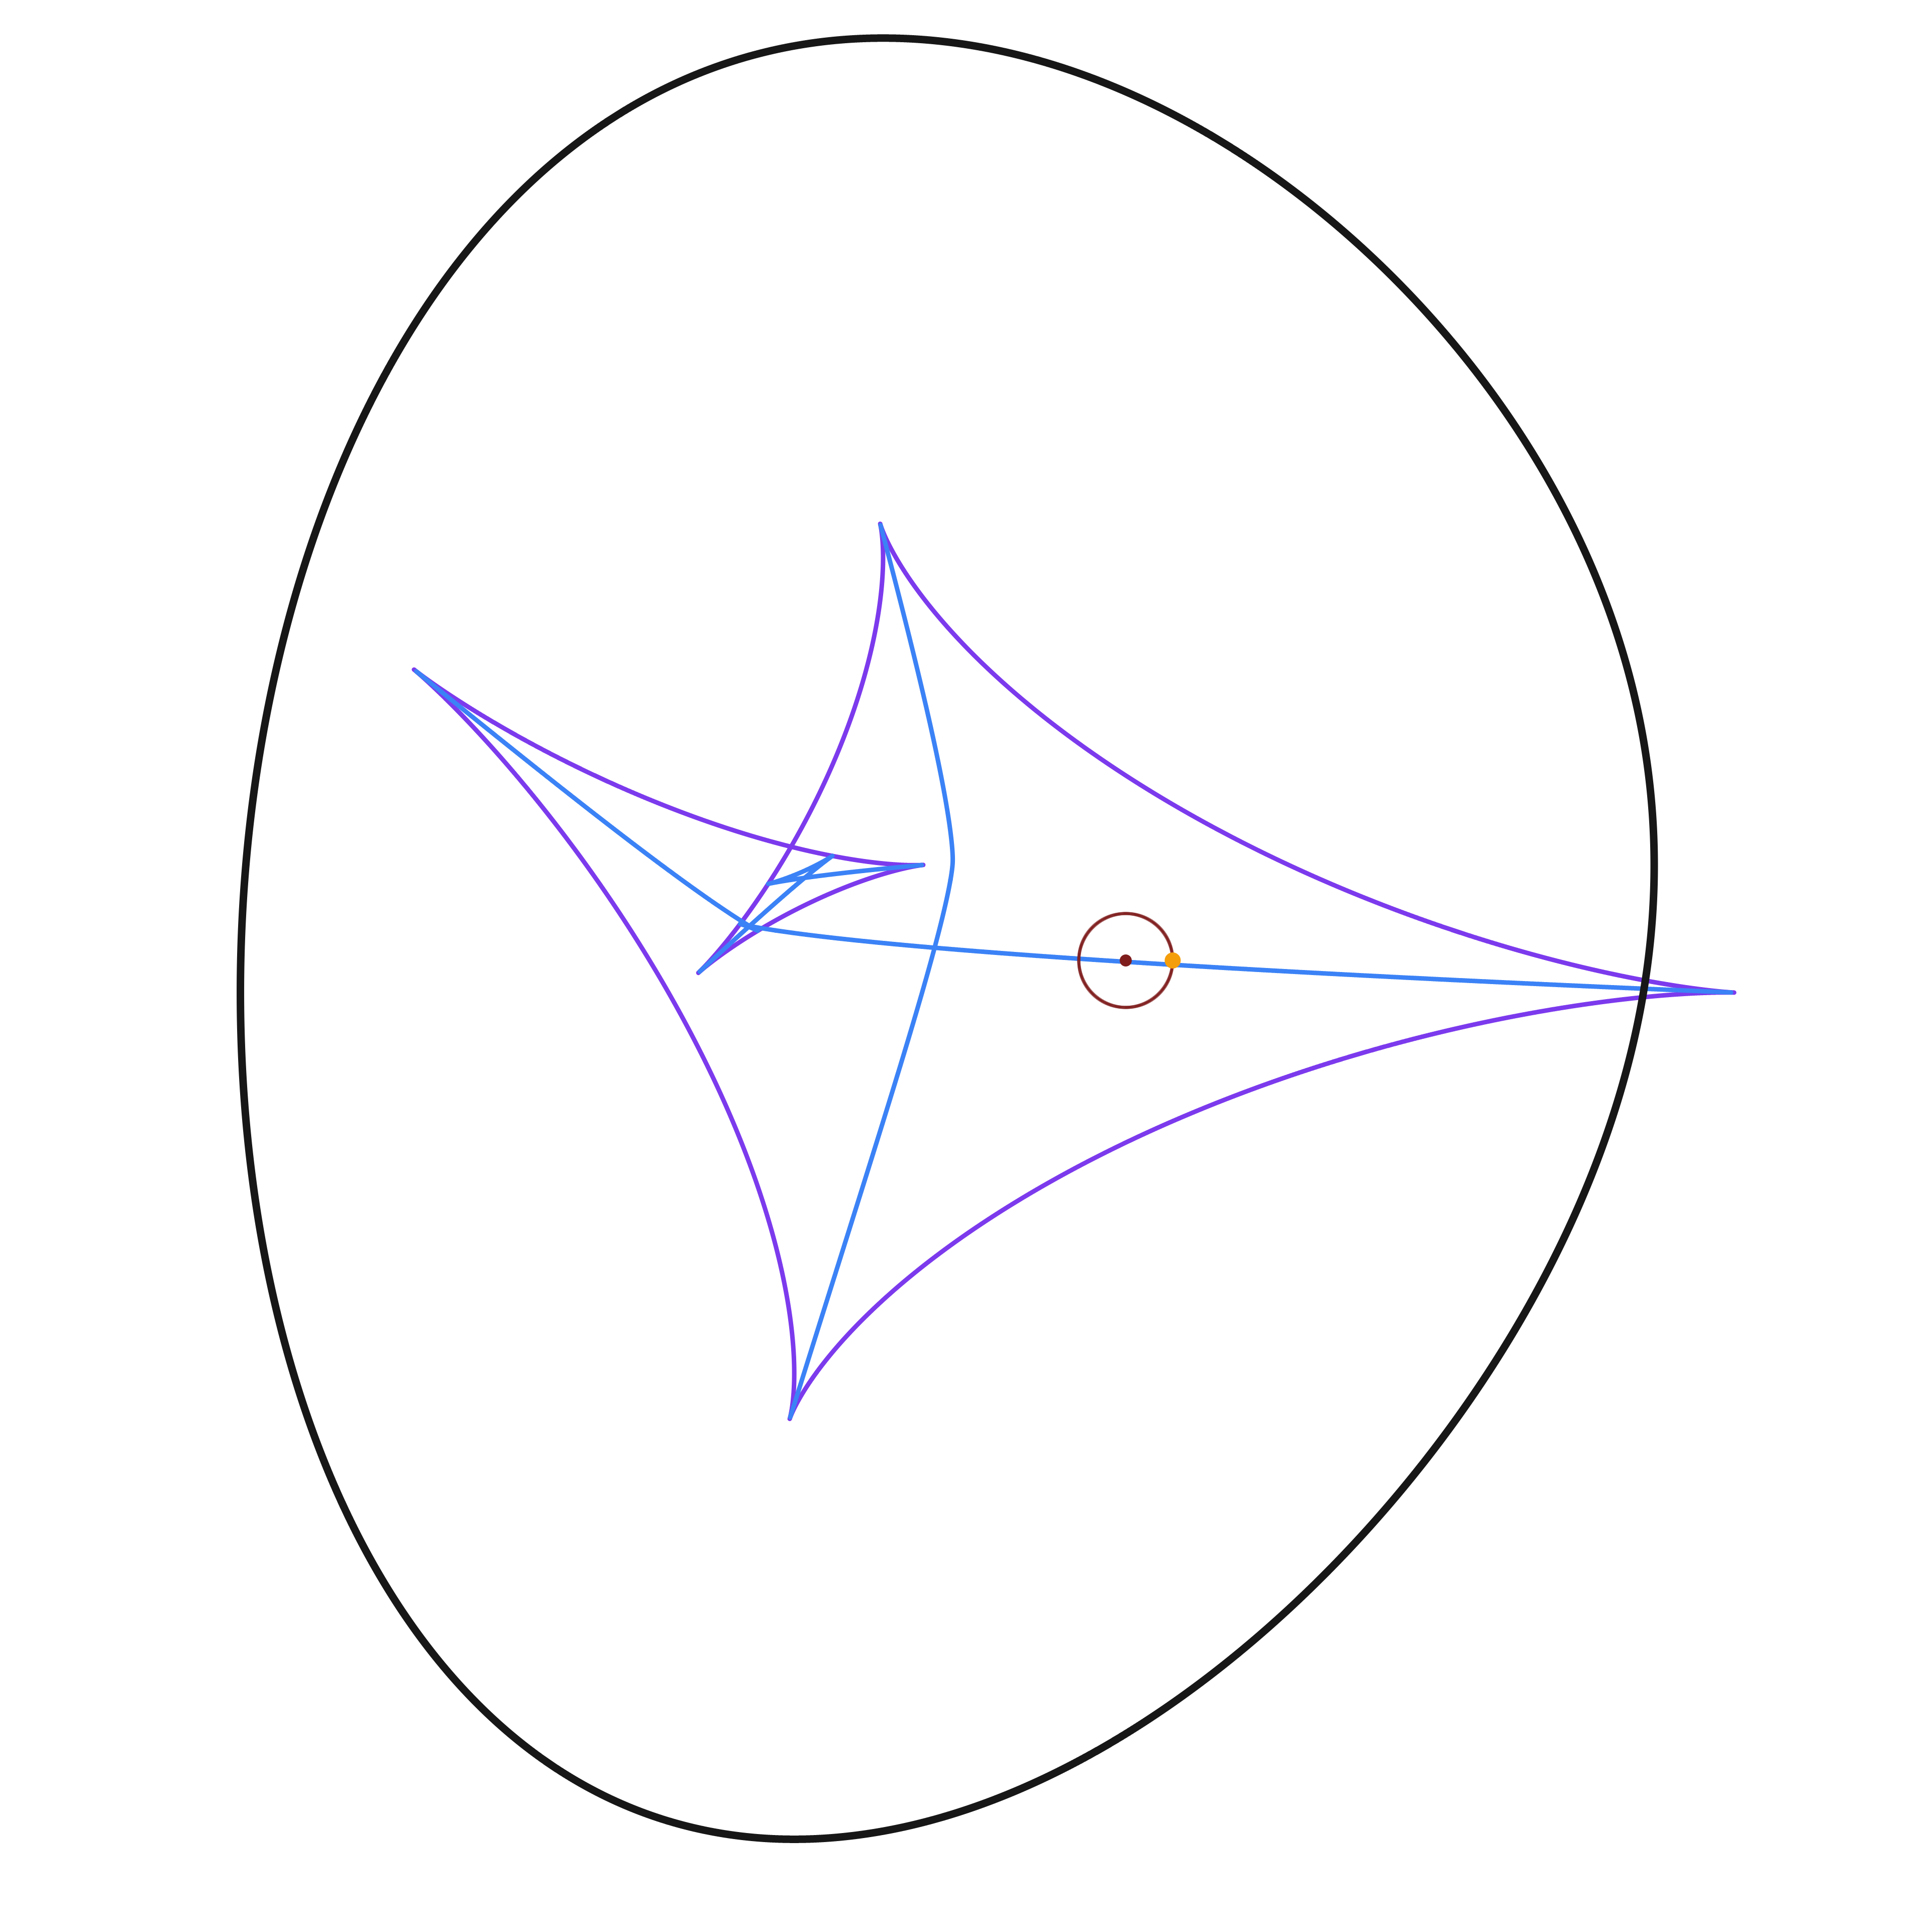
\includegraphics[width=0.32\textwidth]{figures/potato_eg.png}
    \hfill
    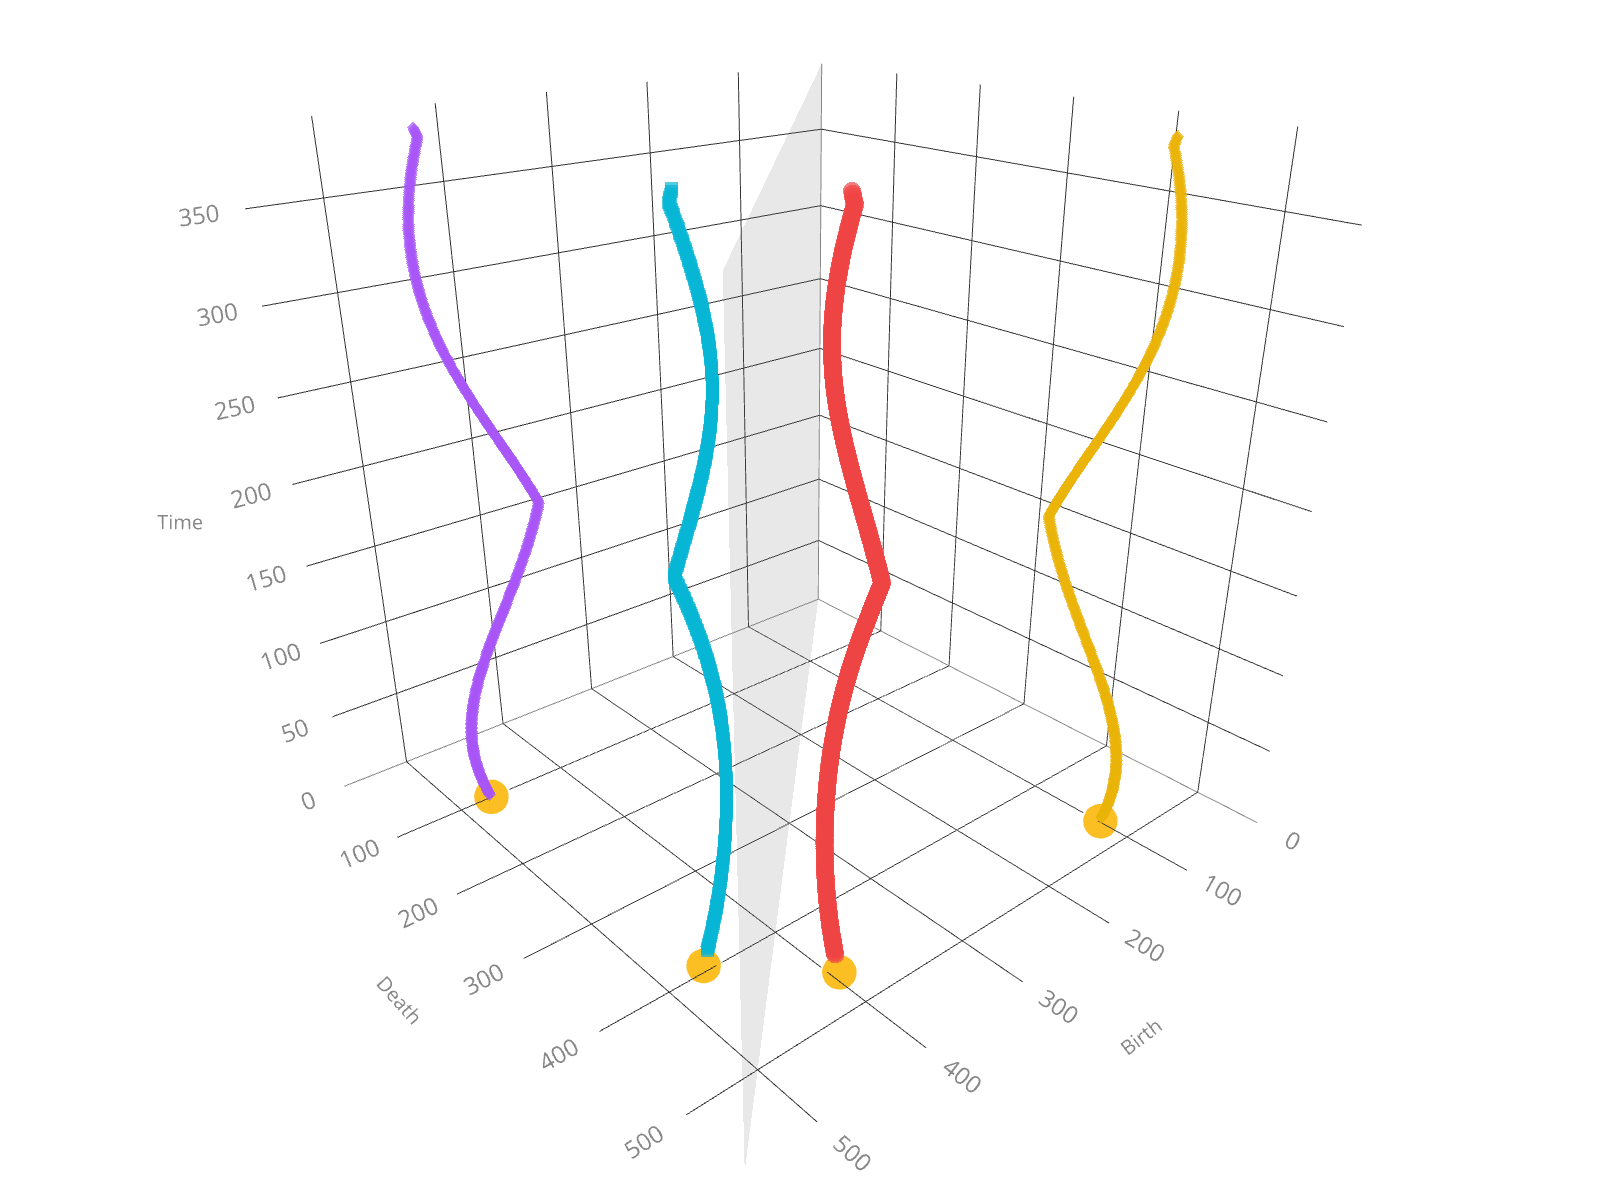
\includegraphics[width=0.36\textwidth]{figures/potato_vin.png}
    \hfill
    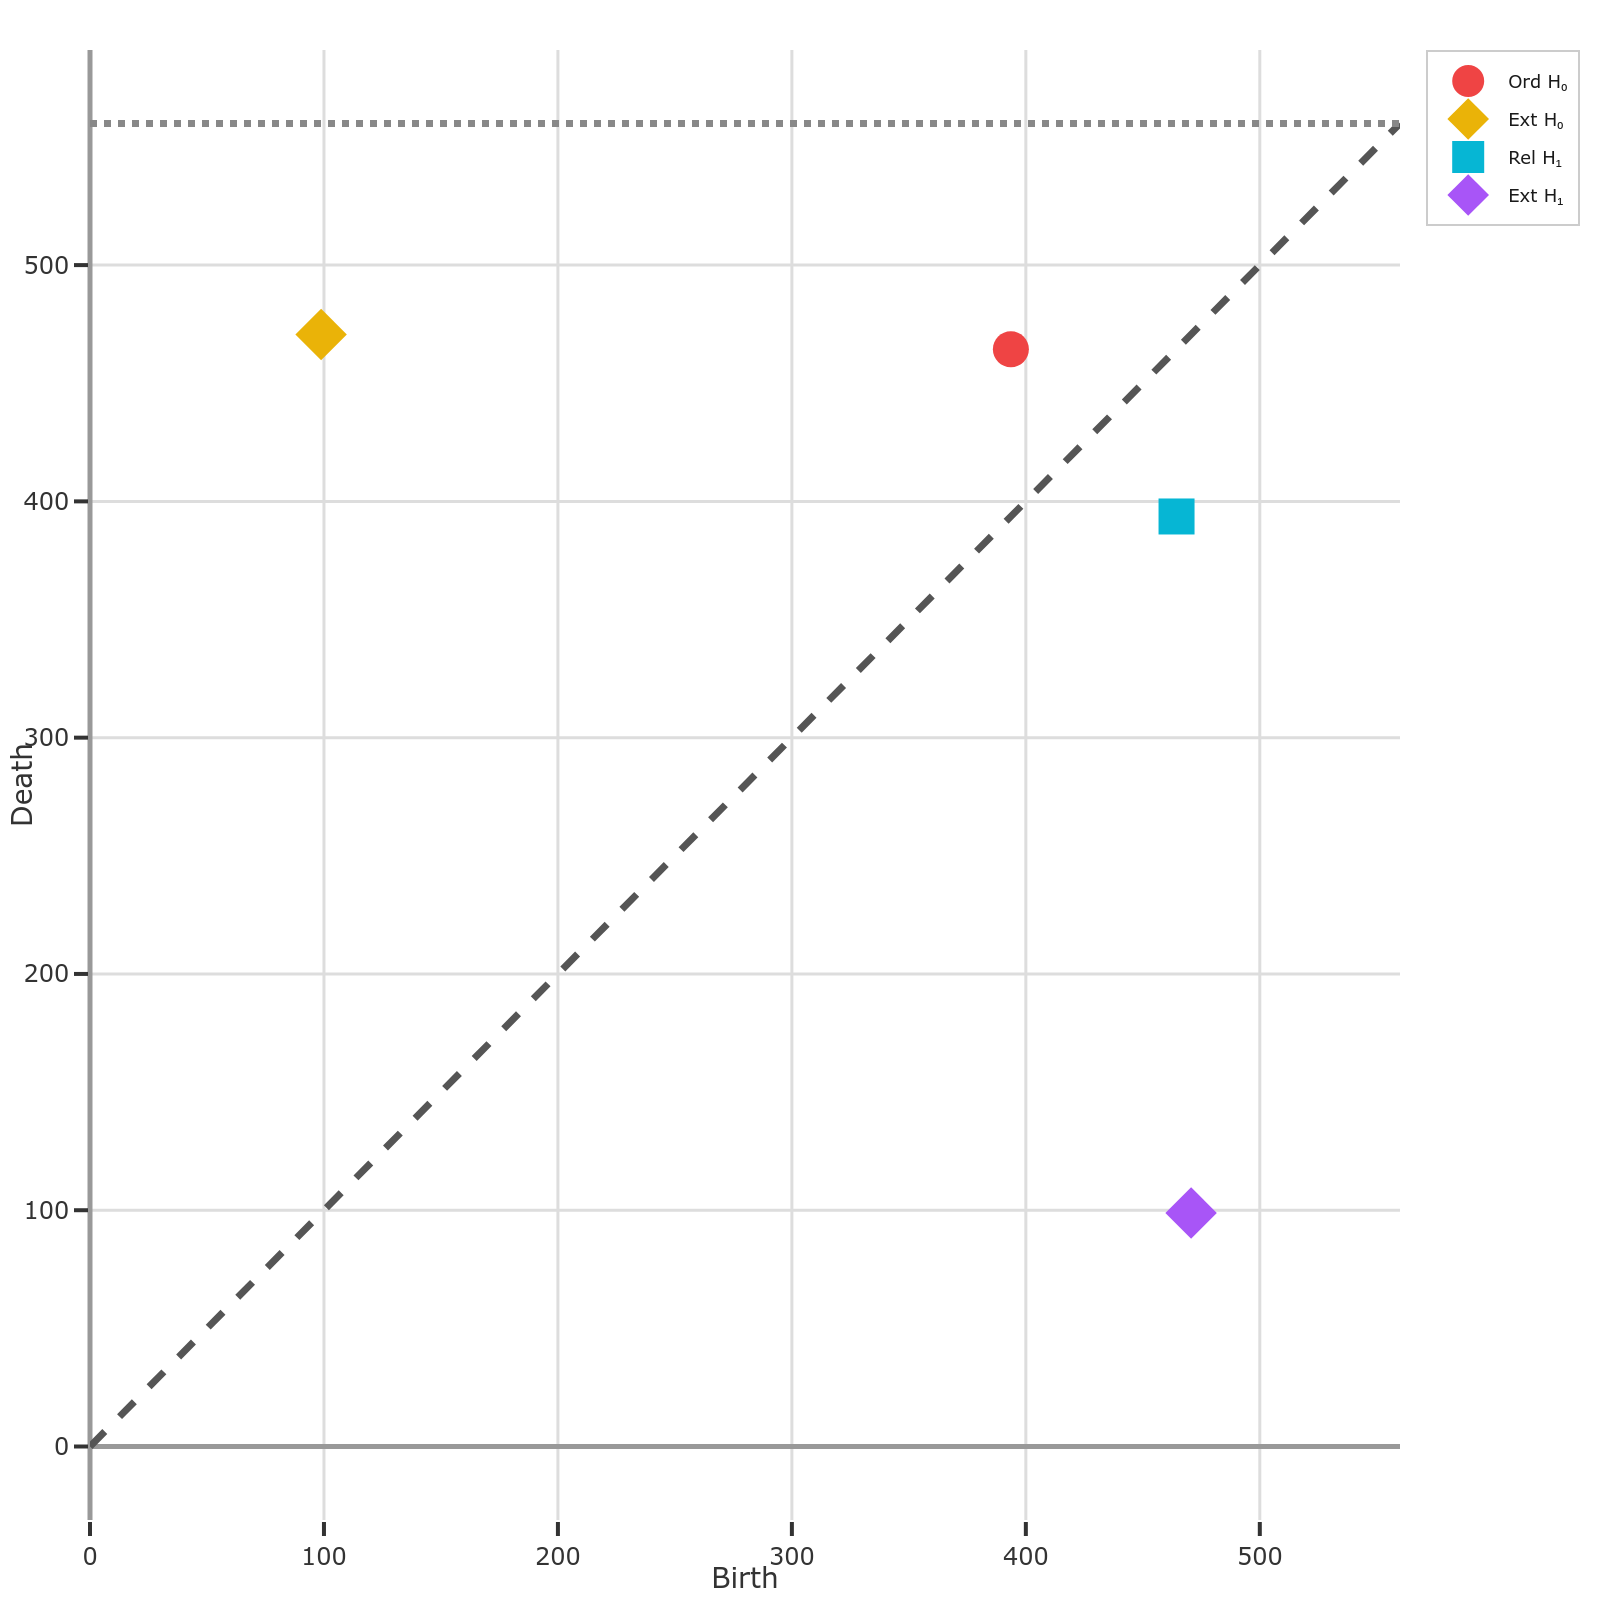
\includegraphics[width=0.29\textwidth]{figures/potato_pd.png}
    \caption{An example of the symmetry (blue) and focal (purple) sets, and a respective vineyard for a potato shaped figure along the reddish-brown loop, and the persistence diagram for the radial filtration for the yellow point.}
    \label{fig:potato_vin}
\end{figure}

\section{Theoretical core: the singular source of monodromy (P3, P2)}

The preprint \textbf{(P3)}, with the short version \textbf{(P2)} presented at CG:YRF, contains the main theoretical results.

\paragraph{Stability outside the generalized symmetry set.}
The first structural result (Proposition~2.7 / Corollary~2.8 in P3) is a stability statement: on any connected component of $\R^2\setminus\gsym(\M)$ the distance function is Morse with distinct critical values, so the persistence pairing is locally constant. Hence a loop that avoids $\gsym(\M)$ produces a vineyard that is simply $k$ unlinked circles with no monodromy, and \emph{all} monodromy must be generated by singularities of $\gsym(\M)$. Moreover only the sequence of components of $\R^2\setminus\gsym(\M)$ that $\gamma$ visits matters for the topology of the vineyard, not the precise geometry of $\gamma$, which allows us to shrink loops around a single singularity without loss of generality.


\paragraph{The interchange mechanism.}
Monodromy arises from an \emph{interchange}: two off-diagonal points whose vines swap places over one period. We show in (P3) that an interchange requires $\gamma$ to cross both a \emph{birth--birth} and a \emph{death--death} stratum of the symmetry set, and hence to involve at least four contact points distributed over exactly two persistence pairs, because for 2 vines to intersect, both their birth and death coordinates have to be the same (again see (P3) for details). As $\gamma$ crosses the symmetry set, two things can happen: the critical values \emph{reorder} (which always occurs), and the persistence \emph{pairing} may change via the elder rule (producing non-smooth points called \emph{knees}). A combination of pairing changes and the orderings is necessary for monodromy to occur.

% \begin{figure}[h!]
% \centering
% \includegraphics[width=0.80\linewidth]{figures/A12_example_cropped.pdf}

% \clearpage
% \caption{A loop $\gamma$ enclosing the symmetry set or an $A_1^2$ singularity (left)  and the associated vineyard (right). There is no monodromy here.}
% \label{fig:A_12 Singularity}
% \end{figure}

\begin{figure}[h!]
    \centering
    \includegraphics[width=0.8\linewidth]{figures/deformed_ellipse_monodromy_new.pdf}
    \caption{Left: The complete symmetry (blue) and focal (purple) sets for the example where a single singularity of type $A_1^2/A_1^2$ generates monodromy. Right: The vineyard exhibiting the monodromy. We stress that the red and turquoise vines do not intersect in three dimensions (the intersection is a result of the projection to the two dimensional paper). %Representation of monodromy for a $A_1^2/A_1^2$ crossing.  \RR{a line to describe this}
    }
    \label{fig:figure3ForA12A12Transition} 
\end{figure} 

\paragraph{Classification.}
The generic (in the sense of Thom, Arnold, and Bruce, Giblin and Gibson~\cite{arnold_singularities,bruce1985symmetry}) planar singularities of $\gsym(\M)$ are classified in Arnold's notation. See Figure \ref{fig:singularities}. Treating each in turn and tracking the reordering/elder-rule effects of a small encircling loop yields a complete verdict:

\begin{figure}[h!]
    \centering
    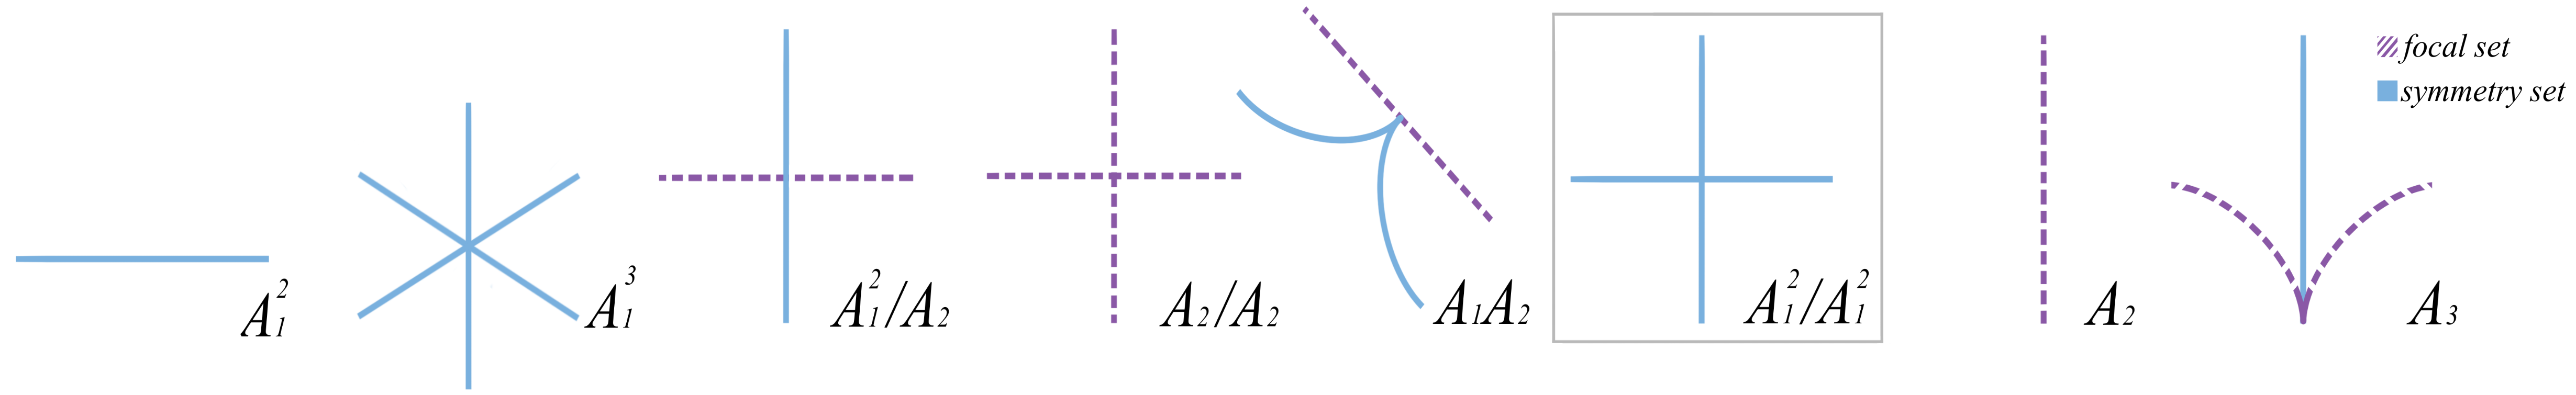
\includegraphics[width=1\linewidth]{figures/symm_line.png}
    \vspace{-2em}
    \caption{The singularities of the symmetry and focal set in the plane. %Representation of monodromy for a $A_1^2/A_1^2$ crossing.  \RR{a line to describe this}
    }
    \label{fig:singularities} 
\end{figure} 


\begin{center}\small
\renewcommand{\arraystretch}{1.15}
\begin{tabular}{@{}llc@{}}
\toprule
Type & Geometric configuration of the circle(s) centred at $p$ & Monodromy \\
\midrule
$A_1^2$       & one circle bitangent to $\M$ (2 contact points) & no \\
$A_1^3$       & one circle tangent at three points              & no \\
$A_1^2/A_1^2$ & two concentric circles, each bitangent (4 contacts) & \textbf{yes} \\
$A_2$         & osculating circle; $p$ on the focal set         & no \\
$A_1A_2$      & one ordinary contact $+$ one second-order contact & no \\
$A_3$         & curvature extremum; cusp of the focal set       & no \\
$A_1^2/A_2$   & concentric bitangent circle $+$ osculating circle & no \\
$A_2/A_2$     & two concentric osculating circles               & no \\
\bottomrule
\end{tabular}
\end{center}

\noindent
% Every ``no'' falls into one of two patterns. The genuine symmetry-set types ($A_1^2$, $A_1^3$) reorder critical values but undo any pairing change as the loop crosses back, and $A_1^3$ simply lacks the four contacts an interchange needs. The focal-set types ($A_2$, $A_1A_2$, $A_3$, $A_1^2/A_2$, $A_2/A_2$) only create and annihilate near-diagonal, self-paired points of very low persistence, which cannot interchange with the established off-diagonal points and so leave the braid trivial. 
In our paper (P3), we perform the extensive analysis which determines in every case whether there can be any monodromy. We stress that very specific configurations are necessary for monodromy to occur. In figure \ref{fig:figure3ForA12A12Transition} we give an example where monodromy occurs thanks to a singularity of type $A_1^2/A_1^2$. We thus have our main result:

\begin{theorem}[P3, P2]
Let $\M \subset \R^2$ be a generic smooth closed curve and $\gamma\colon\Sone\to\R^2$ a generic, sufficiently small loop. If the interior of $\gamma$ contains no singularity of type $A_1^2/A_1^2$ of the symmetry set, then the vineyard $\mathcal V(\M,\gamma)$ has no nontrivial monodromy and consists of $k$ unlinked circles.
\end{theorem}

\paragraph{Significance, a cautionary example and outlook.}
To our knowledge this is the first work to combine the symmetry set, persistent homology, and singularity theory, and it pinpoints the geometric \emph{source} of the topological complexity that earlier work had only constructed. We stress that combinations of monodromy-generating $A_1^2/A_1^2$ singularities do not necessarily combine in large loops to give monodromy as shown in figure \ref{fig:a12a12_bigloop}. It complements two recent results: Chambers et al.\ (\emph{Braiding Vineyards}, SODA~2026)~\cite{chambers2026braiding} showed that closed RPT vineyards can realize arbitrary knots and links, while Arya et al.\ (2024)~\cite{arya2024decomposing} gave conditions excluding monodromy for star-shaped objects. In a manuscript which is being written at the moment, we prove that any large loop that does not contain either singularity of type $A_1^2/A_1^2$ or $A_2/A_2$ does not have monodromy and the vines are unlinked. Large loops that contain a singularity of type $A_2/A_2$ is illustrated in figure \ref{fig:bishop-staff}.

\begin{figure}[h!]
    \centering
    \includegraphics[width=0.9\linewidth]{figures/A12A12_bigloop.pdf}
    \caption{When $\gamma$ is a big enough loop enclosing the curve which acted as an example for a singularity of type $A_1^2/A_1^2$ which contains monodromy, then the vineyard of the larger loop no longer contains monodromy, even though it contains the $A_1^2/A_1^2$ singularity which locally generates monodromy.}
    \label{fig:a12a12_bigloop}
\end{figure}

\begin{figure}
    \centering
    \includegraphics[width=0.65\linewidth]{figures/bishop_staff2.pdf}
    % 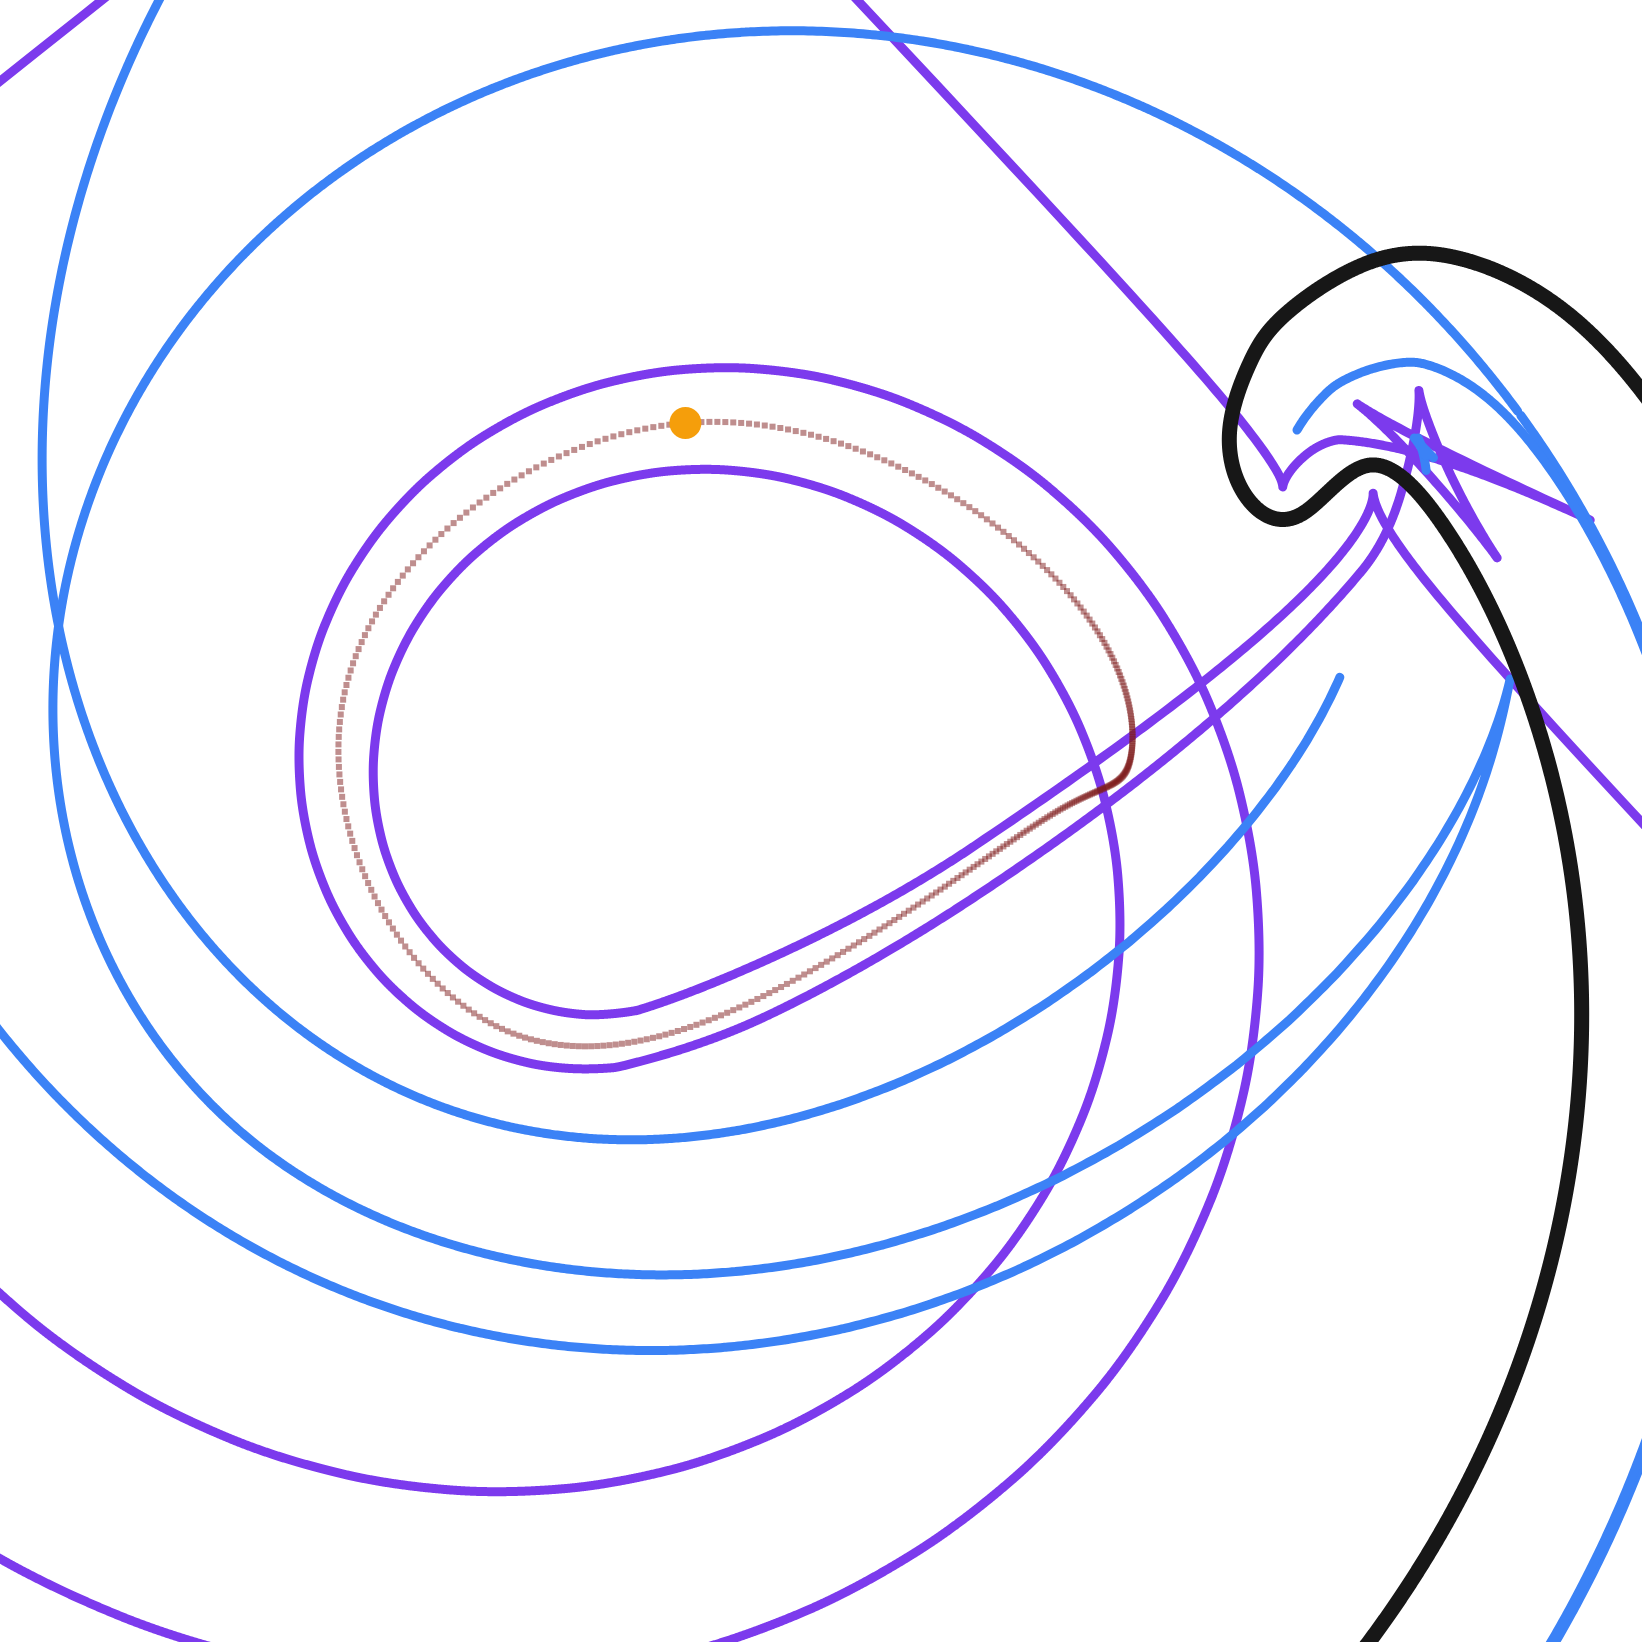
\includegraphics[width=0.3\linewidth]{figures/bishop_zoom.png}
    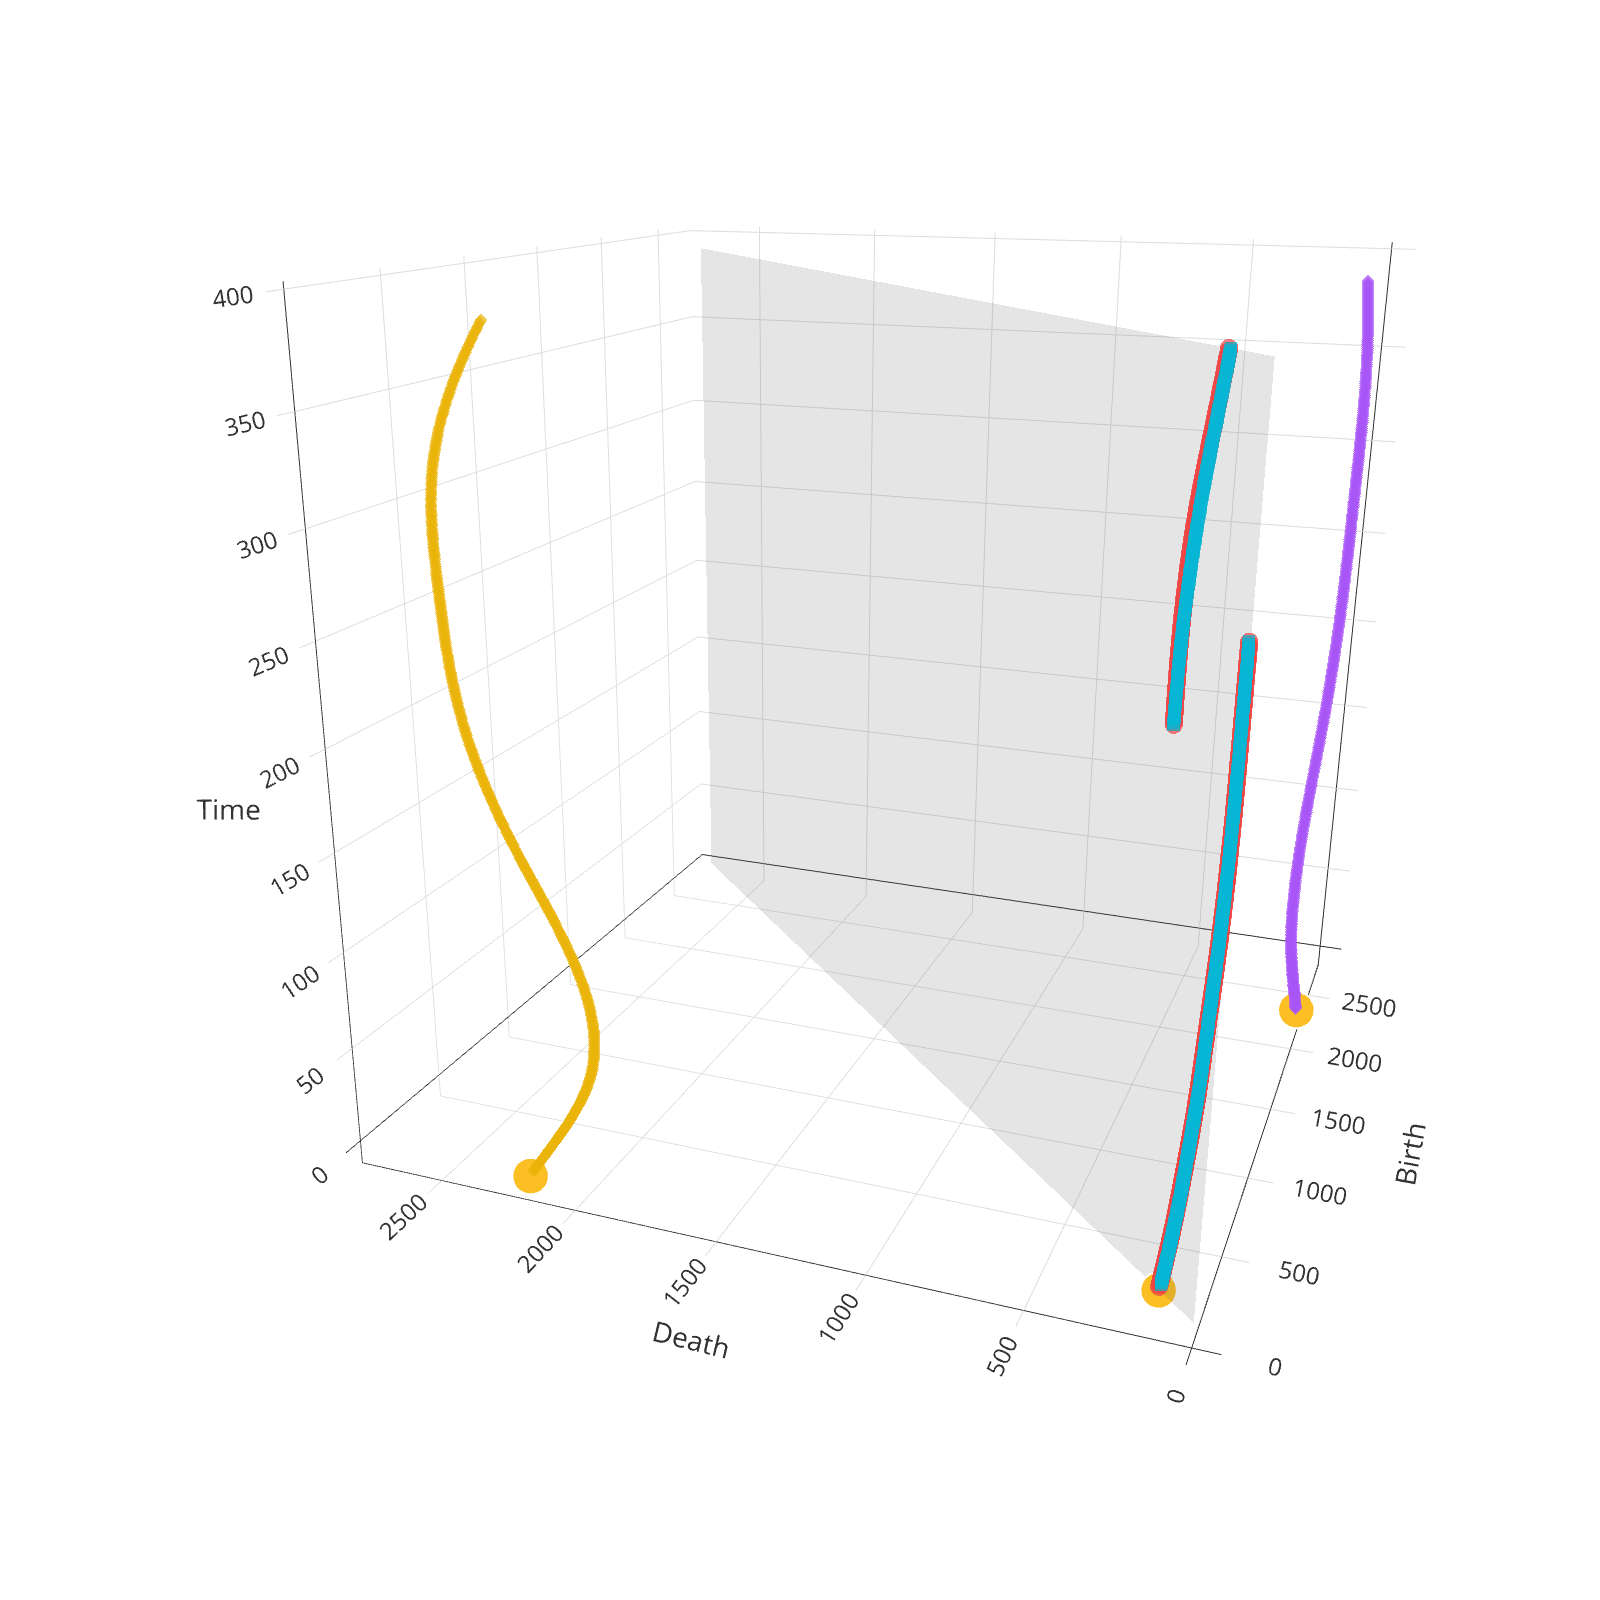
\includegraphics[width=0.34\linewidth]{figures/bishop_vin.png}
    \caption{An example of a bishop staff shaped spiral. A large loop which contains a $A_2/A_2$ singularity, generating monodromy.}
    \label{fig:bishop-staff}
\end{figure}

\section{Software contribution: the Bouquet2D visualization tool (P1)}

The EuroCG paper \textbf{(P1)} introduces \textbf{Bouquet2D} (https://bouquet2d.rohitroy.me), an interactive, web-based tool I developed to explore the geometry above on explicit examples. Given a curve $\M$ defined by an editable spline, the tool computes and renders in real time the focal set (evolute), the symmetry set, and the vineyard of a user-chosen observation loop, which may be a circle of adjustable centre and radius or an arbitrary hand-drawn spline loop.

\paragraph{Algorithms.}
The implementation rests on two pieces. The \emph{symmetry set} is computed as per \cite{bruce1985symmetry} from a sampled curve by detecting sign changes of the bitangency functions $f_\pm(i,j) = (p_i - p_j)\cdot(t_i \pm t_j)$, intersecting the corresponding normal lines, and keeping a candidate centre only when it satisfies an equidistance constraint $\bigl|\,\|C-p_i\|-\|C-p_j\|\,\bigr| < \epsilon_{\mathrm{rad}}$ that suppresses most discretization artifacts. The \emph{vineyard} is assembled by stacking persistence diagrams of the squared distance: for each loop sample a Union--Find pass over the lower-star filtration computes persistence by the elder rule, and the resulting $(t,\text{birth},\text{death})$ triples are tracked into vines. Because the problem is one-dimensional, this elementary approach runs interactively without the more elaborate vineyard-update machinery.

Bouquet2D is publicly available and is offered to the community for feedback; it doubles as a validation engine for the theory and as an exploratory instrument for generating new conjectures. For now, it is limited to smooth planar curves, and its discrete symmetry set computation is sensitive to sampling density, which is set by the user, and to the choice of the constraints (such as $\epsilon_{\mathrm{rad}}$) near singularities.

\section{Triangulations and stratified meshing}

Alongside the vineyard program, and within the StratMesh project, I am implementing the Boissonnat--Kachanovich--Wintraecken algorithm for triangulating submanifolds~\cite{boissonnat2021triangulating}, a quantified, algorithmic version of Whitney's classical construction. Given a compact $C^2$ manifold $\M \subset \R^d$ of positive reach, it uses a perturbed Coxeter triangulation of type $\tilde A_d$ as an ambient scaffold: the vertices are perturbed so that every ambient simplex of dimension at most $d-n-1$ stays away from $\M$, and the triangulation of $\M$ is built by barycentric subdivision of the intersections of $\M$ with the ambient simplices, with explicit quality and Hausdorff bounds and a guaranteed piecewise-smooth homeomorphism. I currently have this working for $1$-manifolds in the plane (curves, codimension one), and $2$-manifolds in $3$-space. 
% The obstruction to higher dimensions is quantitative rather than conceptual: the admissible edge length relative to the reach and the perturbation radii are governed by constants (the $\alpha_k$, $\rho_1$, $\zeta$ of~\cite{boissonnat2021triangulating}) that shrink very fast and depend intricately on the dimension $n$ and codimension $d-n$, making a faithful implementation hard to drive to termination in practice --- which is why progress on higher dimensions is slow.
My numerical experiments have shown that the constants given in \cite{boissonnat2021triangulating} are galactic, in the sense that they are so small to be useless in practice. At the same time, the method works with more reasonable constants. See Figure \ref{fig:torus_triang} for an example. Our goal is to provide implementations up to moderate dimensions ($\leq 5$).
In the longer term this feeds StratMesh's goal of certified meshes for stratified spaces, for which manifold triangulation is a first building block. From there we will go to manifolds with boundary and then manifolds with piecewise smooth boundary, and then stratified spaces, where the strata meet at nice angles and finally stratified spaces with a finite number of types of singularities as the classifications of Thom and Arnold \cite{arnold_singularities}.

\begin{figure}
    \centering
    \fbox{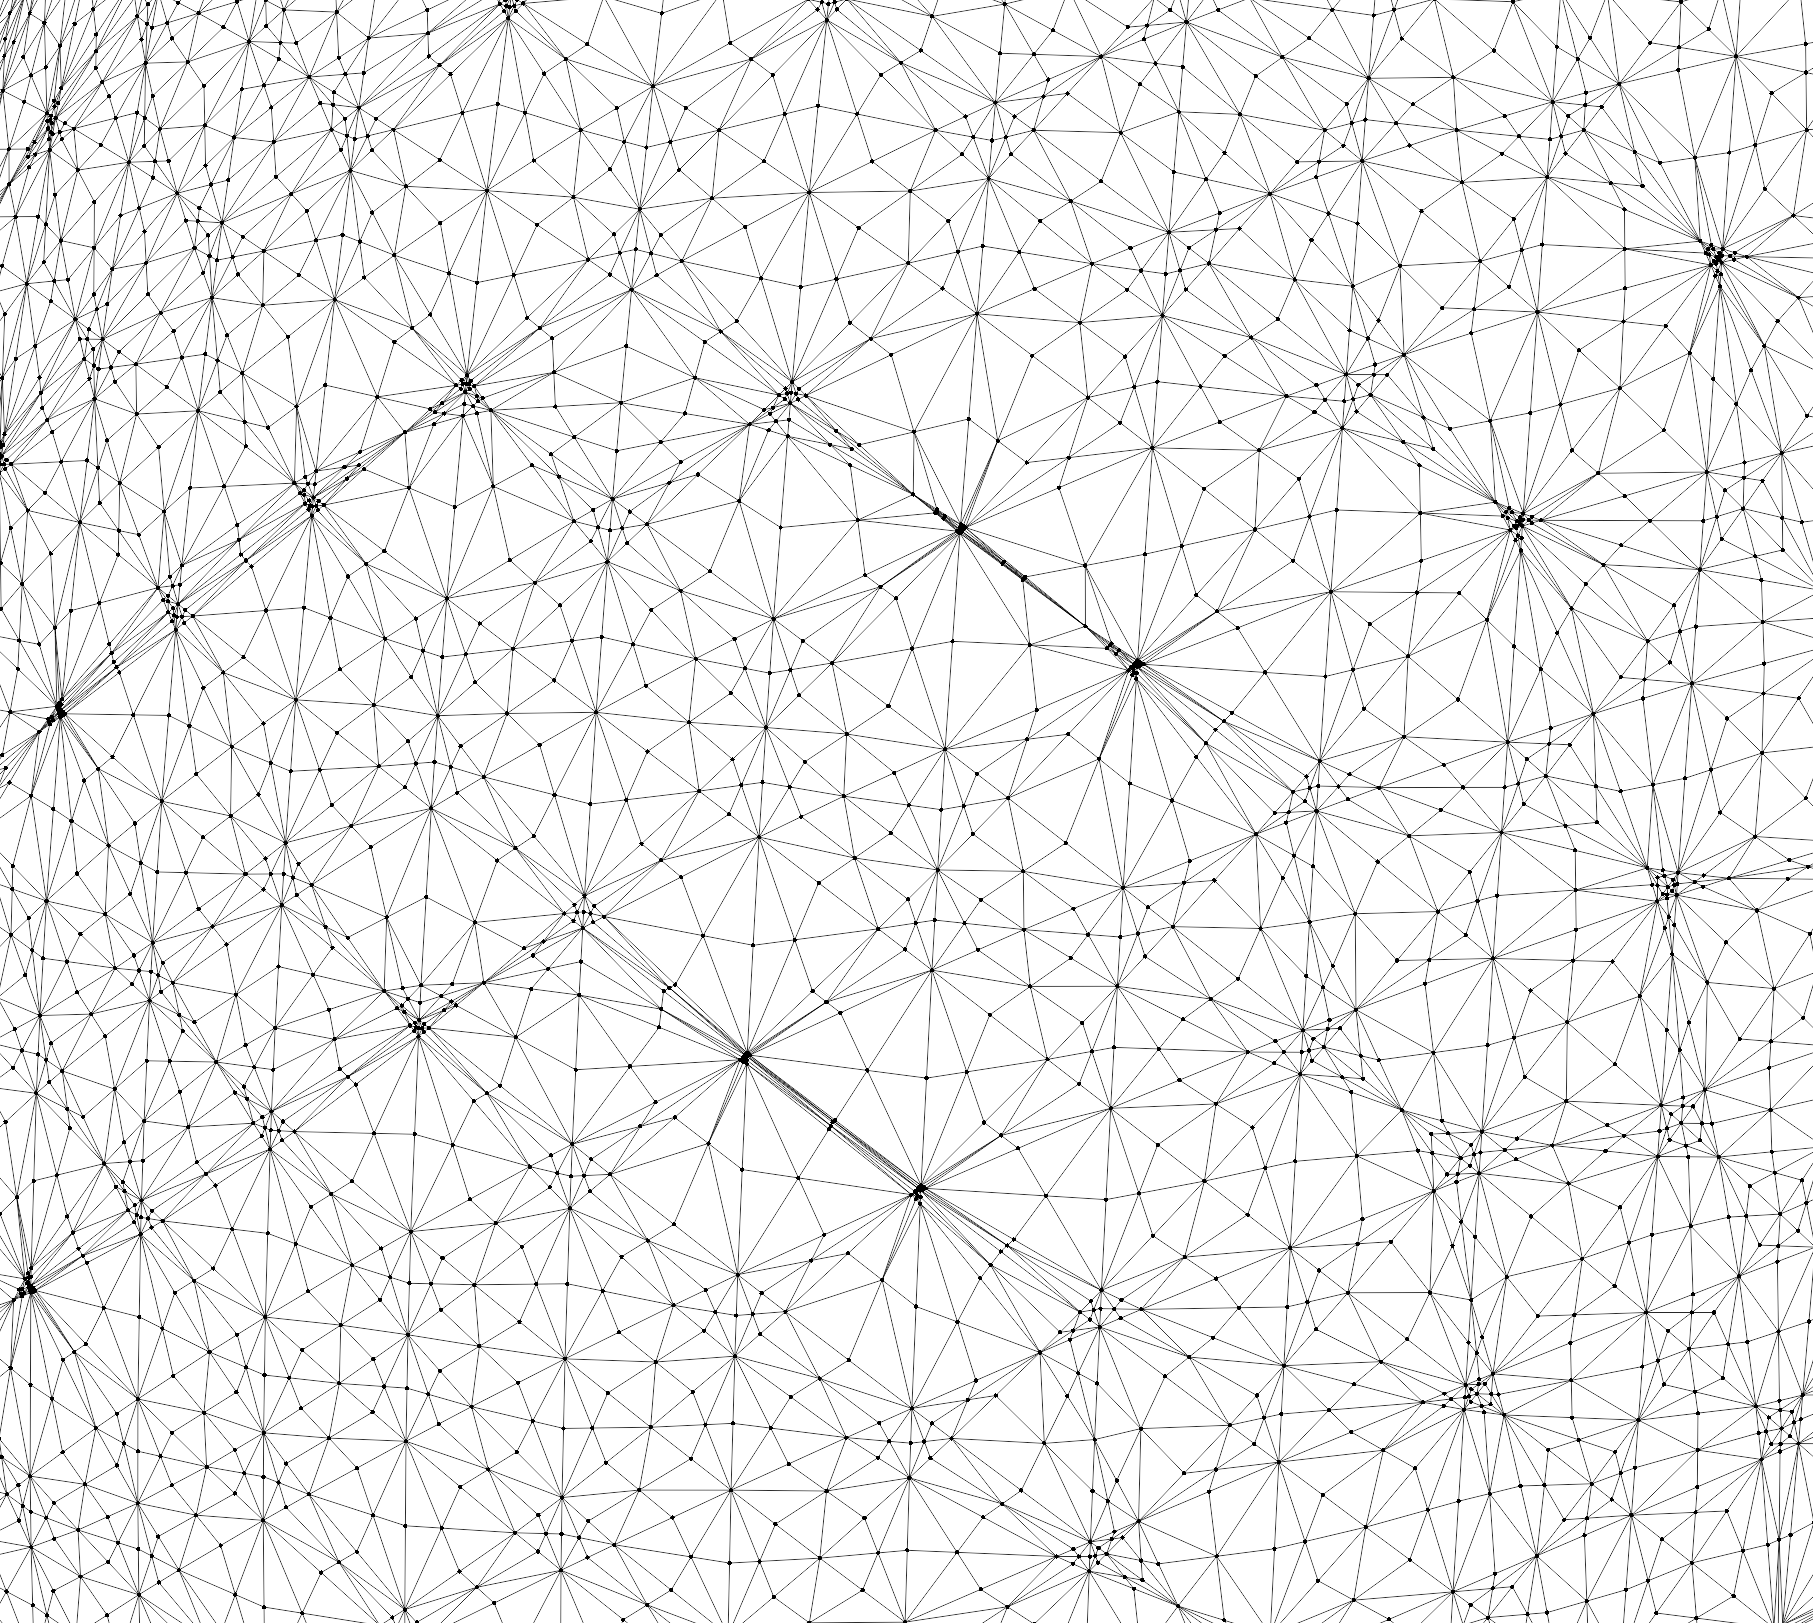
\includegraphics[width=0.45\linewidth]{figures/torus_bad.png}}
    % 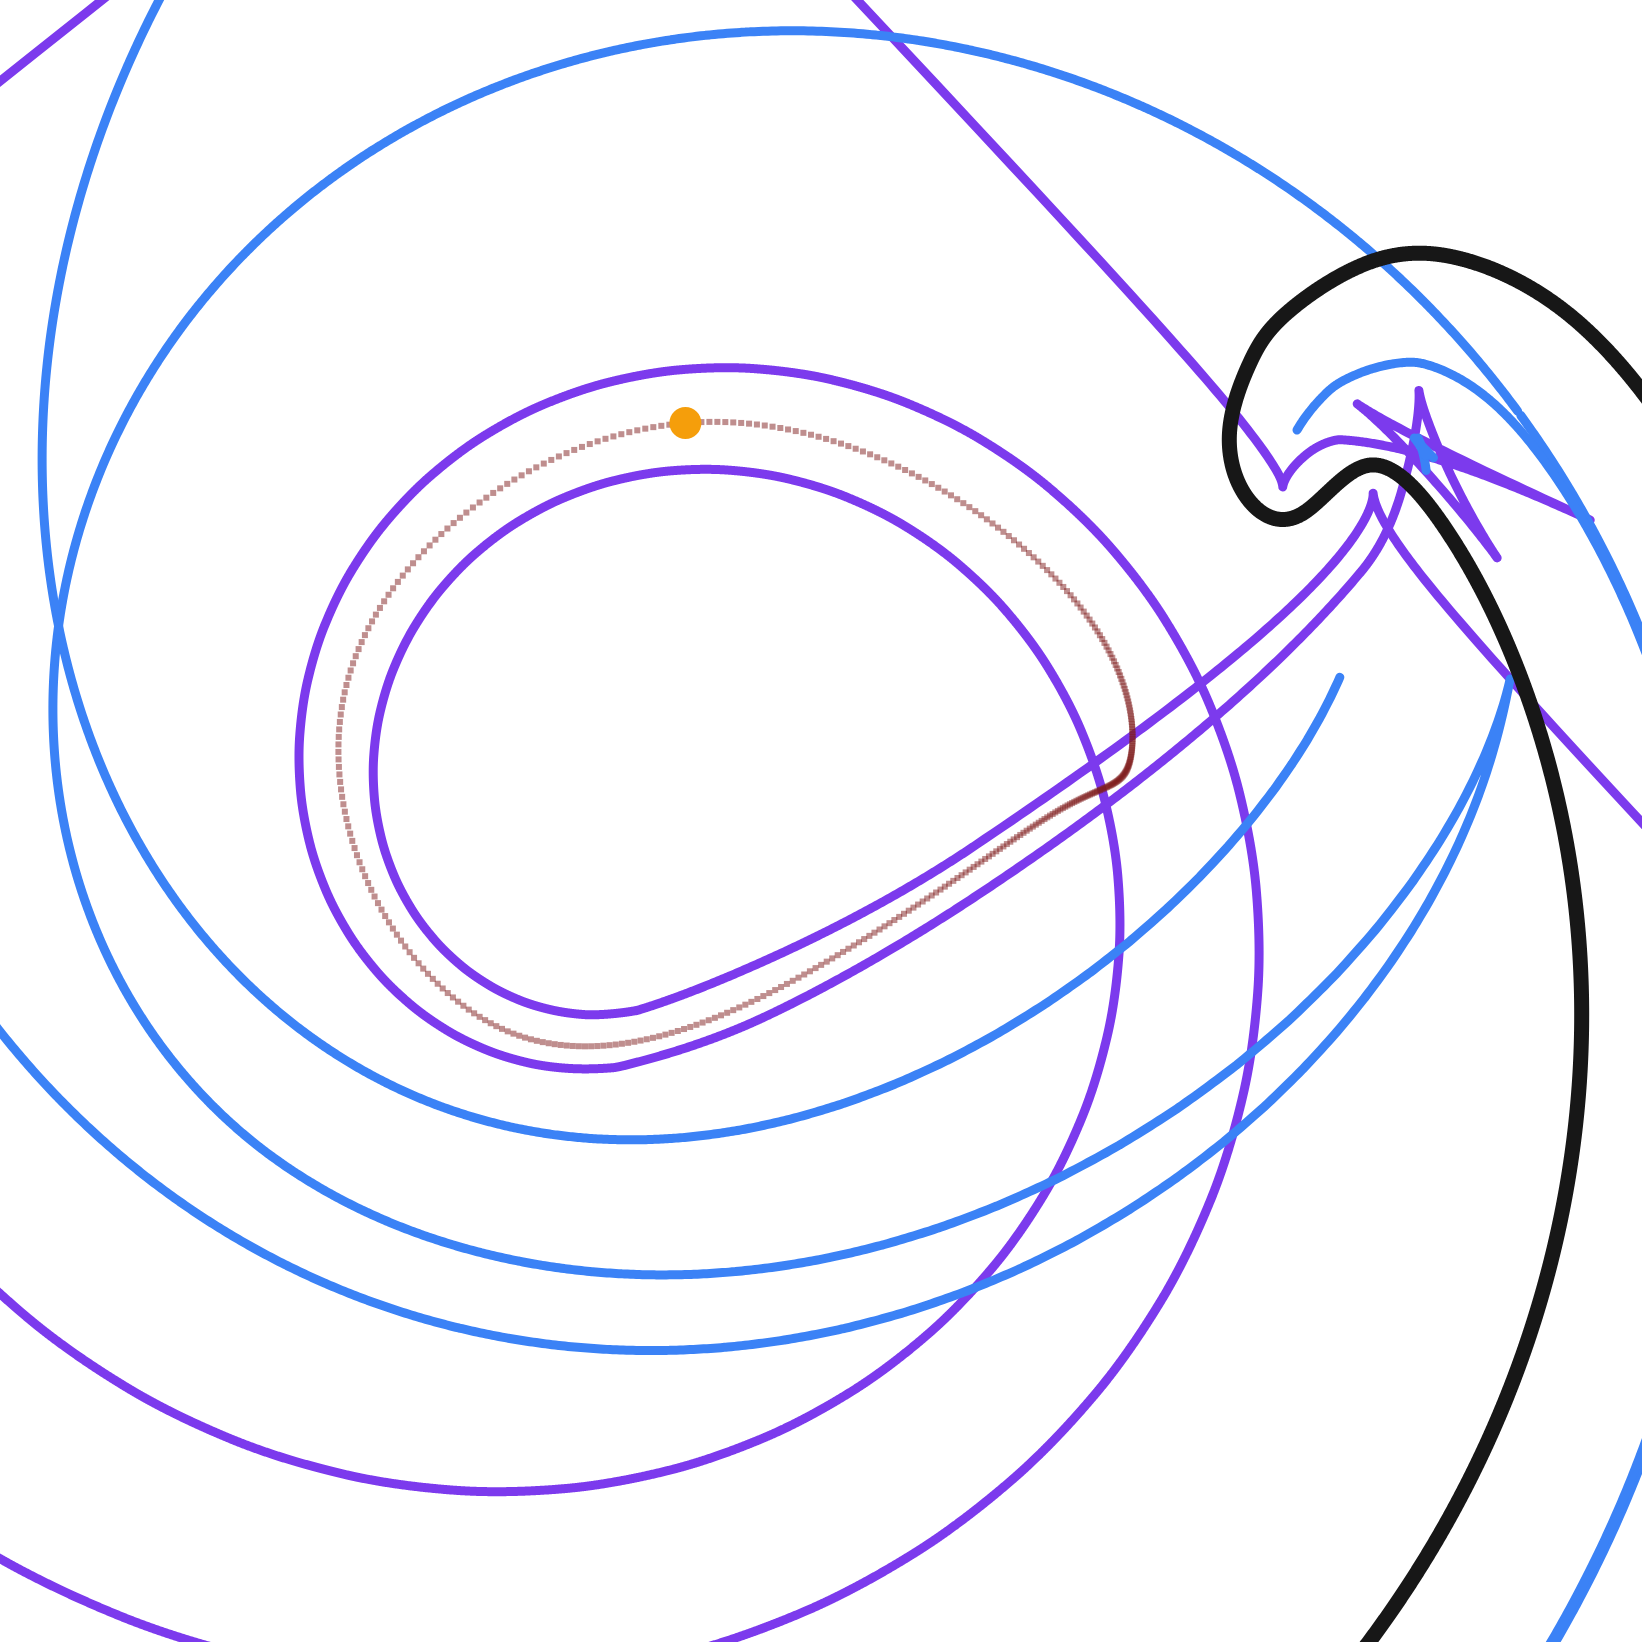
\includegraphics[width=0.3\linewidth]{figures/bishop_zoom.png}
    \hspace{0.5em}
    \fbox{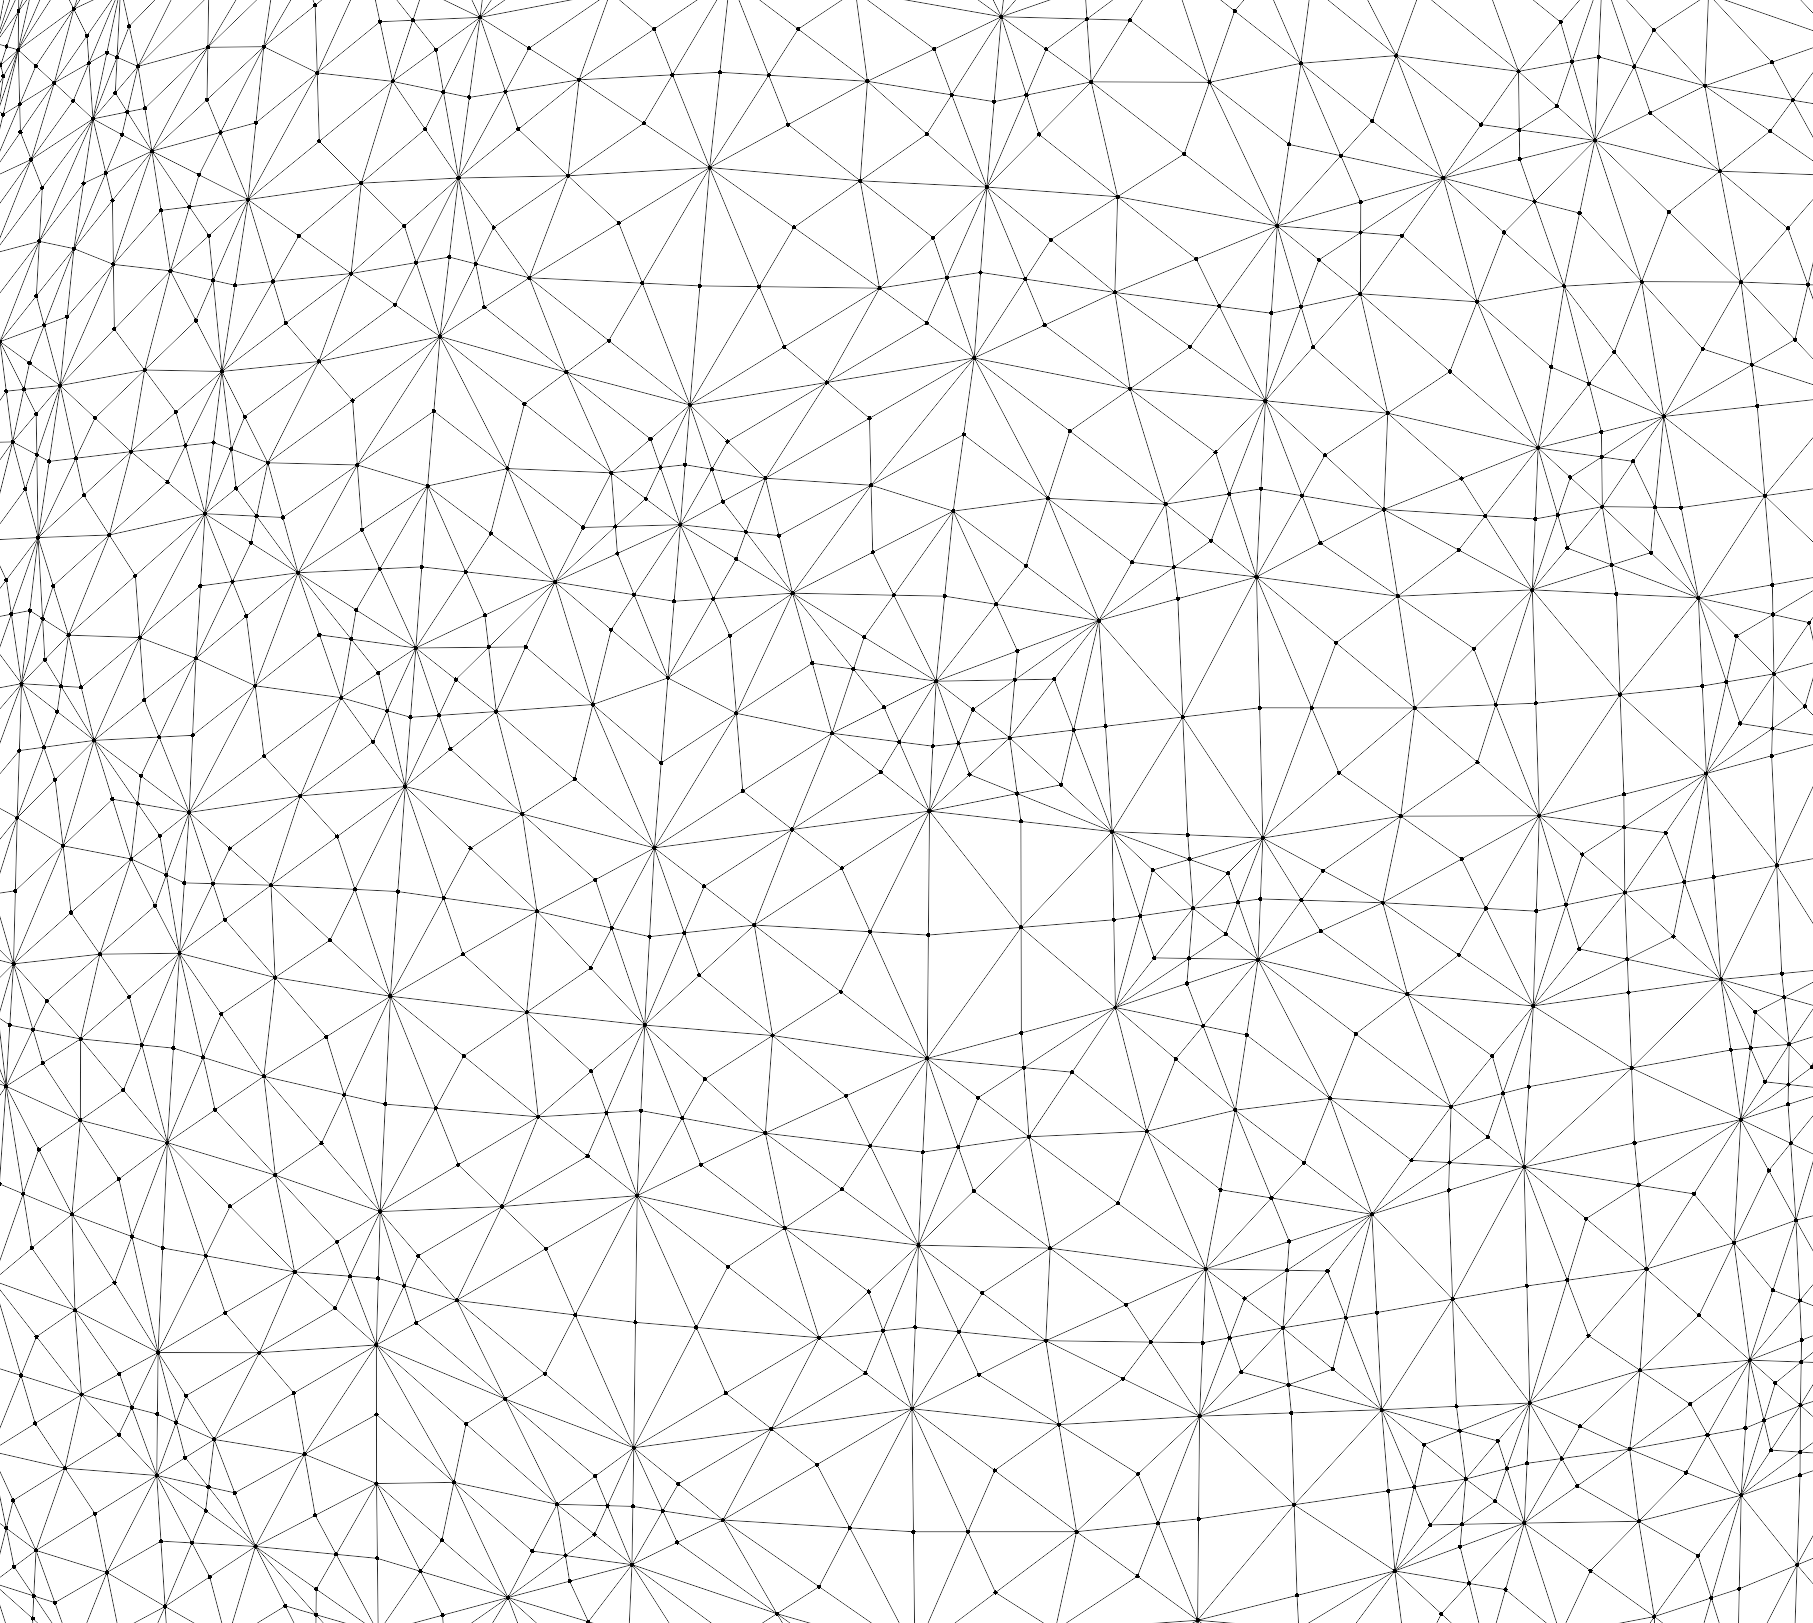
\includegraphics[width=0.45\linewidth]{figures/torus_good.png}}
    \caption{Surface of a torus after the triangulation algorithm of \cite{boissonnat2021triangulating} using constants closer to the paper (left) and with constants much farther away (right).}
    \label{fig:torus_triang}
\end{figure}

\section{Ongoing and future work}

\begin{itemize}
  \item \textbf{Global monodromy criteria.} (Short term) 
  % The local theorem characterizes monodromy for small loops around a single singularity, but its converse fails. The next goal is a criterion that predicts the monodromy of an arbitrary loop --- and its order --- from the sequence of components of $\R^2\setminus\gsym(\M)$ it visits, ideally giving a recipe to build a shape and loop realizing a prescribed order-$k$ monodromy.
  As mentioned above, we are currently extending the local analysis to loops of arbitrary size. 
  \item \textbf{Case Analysis.} (Short term) The precise influence of the singularity of the vineyard also depends heavily on the global topology of $\M$. Currently, we are investigating for which branches near a singularity pairing changes can occur. This gives a classification of the singularities of the $k$-th order medial axis as defined by \cite{edelsbrunner2025mid}.
  \item \textbf{Higher dimensions.} (Mid term) The planar case already contains every singularity essential for loop monodromy, but the eventual target is $\R^3$ and beyond, building on the Bruce--Giblin--Gibson classification of symmetry-set singularities in three dimensions~\cite{bruce1985symmetry}; we expect the two-dimensional structural result to drive that analysis.
  \item \textbf{Stratified meshing.} (Mid to long term) Continued development of the triangulation work toward certified meshes of stratified spaces under StratMesh.
\end{itemize}

\pagebreak
\section*{Publications and preprints}
{\footnotesize
\begin{enumerate}[label={[\arabic*]},leftmargin=2.2em]
  \item E.~W.~Chambers, C.~Fillmore, S.~S.~Mukherjee, R.~Roy, E.~Stephenson, M.~Wintraecken. \emph{Bouquet: A Visualization Tool for Symmetry Sets and Vineyards.} EuroCG 2026 -- 42nd European Workshop on Computational Geometry, Hagen, Germany, 2026. URL: https://hal.science/hal-05546179
  \item E.~Chambers, C.~Fillmore, S.~S.~Mukherjee, R.~Roy, E.~Stephenson, M.~Wintraecken. \emph{The symmetry set as a knitting pattern for vineyards.} Computational Geometry: Young Researchers Forum (CG:YRF), 2026.
  \item E.~W.~Chambers, C.~Fillmore, S.~S.~Mukherjee, R.~Roy, E.~Stephenson, M.~Wintraecken. \emph{The Singular Source of Vineyard Monodromy,} 2026. Preprint, arXiv:2607.01046 (submitted to SODA).
\end{enumerate}
}

\renewcommand{\refname}{Selected references}
\nocite{*}
{\footnotesize
\bibliographystyle{plain}
\bibliography{references}
}

\end{document}